%% bare_jrnl.tex
%% V1.4b
%% 2015/08/26
%% by Michael Shell
%% see http://www.michaelshell.org/
%% for current contact information.
%%
%% This is a skeleton file demonstrating the use of IEEEtran.cls
%% (requires IEEEtran.cls version 1.8b or later) with an IEEE
%% journal paper.
%%
%% Support sites:
%% http://www.michaelshell.org/tex/ieeetran/
%% http://www.ctan.org/pkg/ieeetran
%% and
%% http://www.ieee.org/

%%*************************************************************************
%% Legal Notice:
%% This code is offered as-is without any warranty either expressed or
%% implied; without even the implied warranty of MERCHANTABILITY or
%% FITNESS FOR A PARTICULAR PURPOSE!
%% User assumes all risk.
%% In no event shall the IEEE or any contributor to this code be liable for
%% any damages or losses, including, but not limited to, incidental,
%% consequential, or any other damages, resulting from the use or misuse
%% of any information contained here.
%%
%% All comments are the opinions of their respective authors and are not
%% necessarily endorsed by the IEEE.
%%
%% This work is distributed under the LaTeX Project Public License (LPPL)
%% ( http://www.latex-project.org/ ) version 1.3, and may be freely used,
%% distributed and modified. A copy of the LPPL, version 1.3, is included
%% in the base LaTeX documentation of all distributions of LaTeX released
%% 2003/12/01 or later.
%% Retain all contribution notices and credits.
%% ** Modified files should be clearly indicated as such, including  **
%% ** renaming them and changing author support contact information. **
%%*************************************************************************


% *** Authors should verify (and, if needed, correct) their LaTeX system  ***
% *** with the testflow diagnostic prior to trusting their LaTeX platform ***
% *** with production work. The IEEE's font choices and paper sizes can   ***
% *** trigger bugs that do not appear when using other class files.       ***                          ***
% The testflow support page is at:
% http://www.michaelshell.org/tex/testflow/



\documentclass[journal]{IEEEtran}
%
% If IEEEtran.cls has not been installed into the LaTeX system files,
% manually specify the path to it like:
% \documentclass[journal]{../sty/IEEEtran}





% Some very useful LaTeX packages include:
% (uncomment the ones you want to load)


% *** MISC UTILITY PACKAGES ***
%
%\usepackage{ifpdf}
% Heiko Oberdiek's ifpdf.sty is very useful if you need conditional
% compilation based on whether the output is pdf or dvi.
% usage:
% \ifpdf
%   % pdf code
% \else
%   % dvi code
% \fi
% The latest version of ifpdf.sty can be obtained from:
% http://www.ctan.org/pkg/ifpdf
% Also, note that IEEEtran.cls V1.7 and later provides a builtin
% \ifCLASSINFOpdf conditional that works the same way.
% When switching from latex to pdflatex and vice-versa, the compiler may
% have to be run twice to clear warning/error messages.
\usepackage{hyperref}
\hypersetup{
  colorlinks=true,
  urlcolor=blue
}
\usepackage{multicol,caption}
\newenvironment{Figure}
  {\par\medskip\noindent\minipage{\linewidth}}
  {\endminipage\par\medskip}





% *** CITATION PACKAGES ***
%
%\usepackage{cite}
% cite.sty was written by Donald Arseneau
% V1.6 and later of IEEEtran pre-defines the format of the cite.sty package
% \cite{} output to follow that of the IEEE. Loading the cite package will
% result in citation numbers being automatically sorted and properly
% "compressed/ranged". e.g., [1], [9], [2], [7], [5], [6] without using
% cite.sty will become [1], [2], [5]--[7], [9] using cite.sty. cite.sty's
% \cite will automatically add leading space, if needed. Use cite.sty's
% noadjust option (cite.sty V3.8 and later) if you want to turn this off
% such as if a citation ever needs to be enclosed in parenthesis.
% cite.sty is already installed on most LaTeX systems. Be sure and use
% version 5.0 (2009-03-20) and later if using hyperref.sty.
% The latest version can be obtained at:
% http://www.ctan.org/pkg/cite
% The documentation is contained in the cite.sty file itself.






% *** GRAPHICS RELATED PACKAGES ***
%
\ifCLASSINFOpdf
  \usepackage[pdftex]{graphicx}
  % declare the path(s) where your graphic files are
  % \graphicspath{{../pdf/}{../jpeg/}}
  % and their extensions so you won't have to specify these with
  % every instance of \includegraphics
  % \DeclareGraphicsExtensions{.pdf,.jpeg,.png}
\else
  % or other class option (dvipsone, dvipdf, if not using dvips). graphicx
  % will default to the driver specified in the system graphics.cfg if no
  % driver is specified.
  % \usepackage[dvips]{graphicx}
  % declare the path(s) where your graphic files are
  % \graphicspath{{../eps/}}
  % and their extensions so you won't have to specify these with
  % every instance of \includegraphics
  % \DeclareGraphicsExtensions{.eps}
\fi


% correct bad hyphenation here
\hyphenation{op-tical net-works semi-conduc-tor}


\begin{document}
%
% paper title
% Titles are generally capitalized except for words such as a, an, and, as,
% at, but, by, for, in, nor, of, on, or, the, to and up, which are usually
% not capitalized unless they are the first or last word of the title.
% Linebreaks \\ can be used within to get better formatting as desired.
% Do not put math or special symbols in the title.
\title{Microjuego Asteroids GDD}
\author{Alexander Zerpa, c200339}
\maketitle

\section*{Escenas}

Solo existe una escena, \textit{MainScene} en donde se encuentran todos los
\textit{GameObjects} y en donde ocurre la enteridad del juego.

% \hfill Put the date OF WRITING in here in the format: June 02, 2018

\section*{Assets y GameObjects}

\subsection*{GameObjects:}

\begin{multicols}{2}
  \subsubsection*{Space}
  Sprite simple que representa el fondo del área del juego.

  \vfill\null
  \columnbreak

  \begin{Figure}
    \centering
    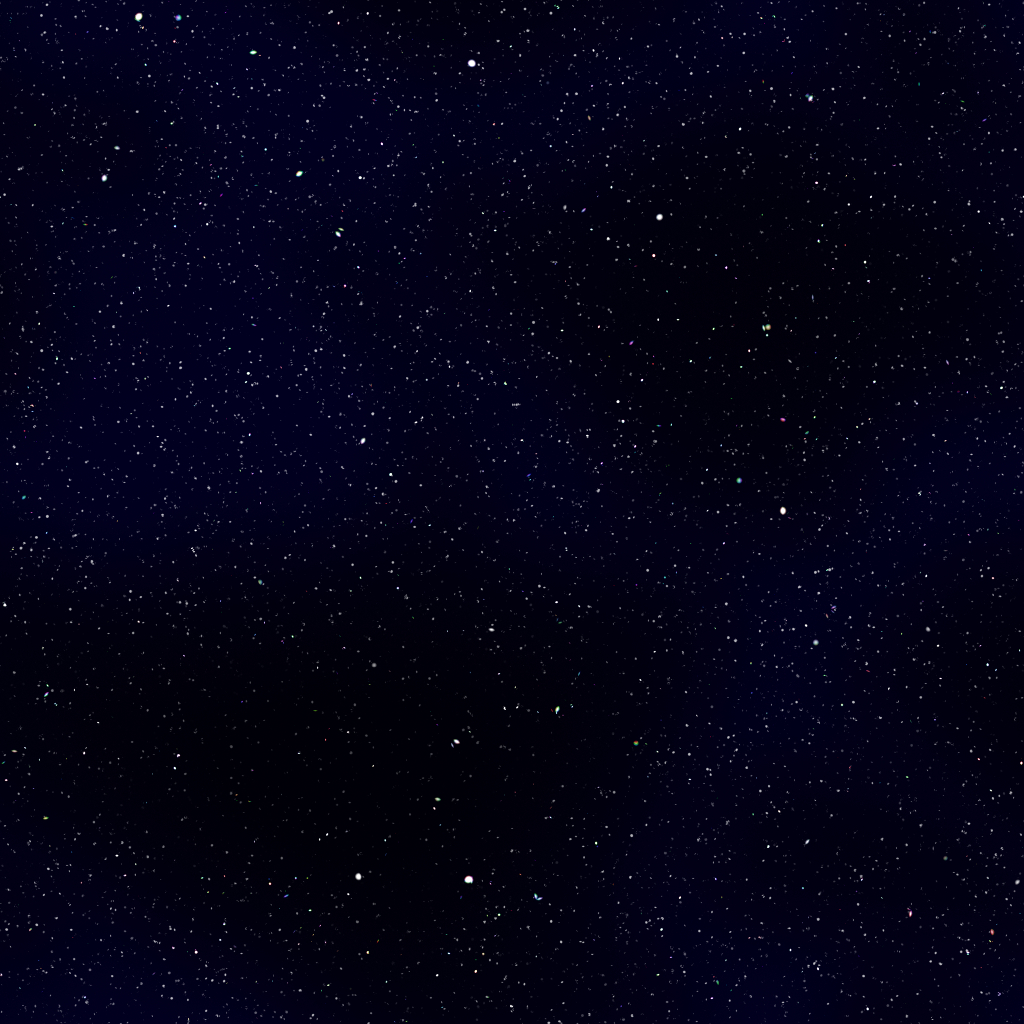
\includegraphics[width=0.3\linewidth]{../Assets/Sprites/Space.jpg}
    \captionof{figure}{Space sprite}
    \label{fig:SpaceSprite}
  \end{Figure}
  \vfill\null
\end{multicols}


\begin{multicols}{2}
  \subsubsection*{Ship}
  Sprite simple con colisiones y lógica, representa al jugador.

  \medskip
  \paragraph*{BulletSpawner}
  Anidado dentro de \textit{Ship}, usado para el spawn de \textit{Bullet}.

  \vfill\null
  \columnbreak

  \begin{Figure}
    \centering
    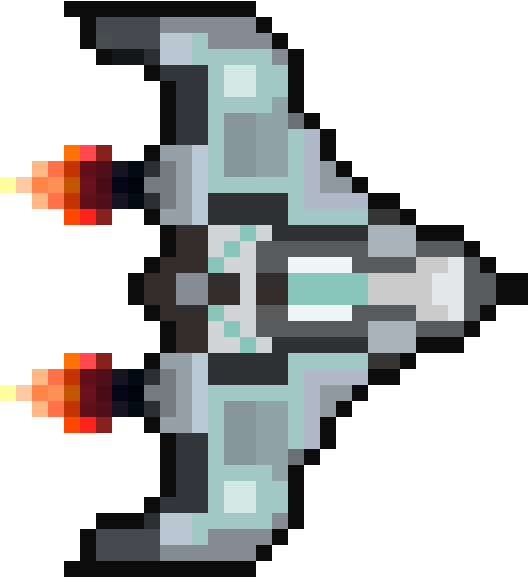
\includegraphics[width=0.4\linewidth]{../Assets/Sprites/Ship.png}
    \captionof{figure}{Ship sprite}
    \label{fig:ShipSprite}
  \end{Figure}
  \vfill\null
\end{multicols}


\subsubsection*{Canvas}
Contiene los elementos de UI.
\paragraph*{Score}
Texto que indica la puntuacion del jugador.
\paragraph*{PauseButton}
Se usa para pausar el juego.

\medskip
\subsubsection*{MainCamera}
Usada para el renderizado del juego.

\medskip
\subsubsection*{EventSystem}
Autogenerado por Unity.

\subsection*{Prefabs:}

\subsubsection*{Bullet}
Spawneado por \textit{BulletSpawner}, tiene colisionador y logica propia.

\begin{multicols}{2}
  \subsubsection*{Meteor}
  Principal enemigo del juego, al ser impactado por \textit{Bullet} es
  reemplazado por dos \textit{MeteorSmall}.

  \medskip

  \subsubsection*{MeteorSmall}
  Igual que \textit{Meteor} solo que mas pequeño y con logica de movimiento
  manejada por script.

  \vfill\null
  \columnbreak

  \null\vfill
  \begin{Figure}
    \centering
    
\includegraphics[width=0.4\linewidth]{../Assets/Sprites/Meteor.png}
    \captionof{figure}{Meteor sprite}
    \label{fig:MeteorSprite}
  \end{Figure}
  \vfill\null
\end{multicols}

\break


\section*{Mecánicas}

\subsection*{Movimiento}
El jugador se mueve controlando la aceleración de la nave y su rotación.

\subsubsection*{Looping}
Si el jugador se desplaza fuera de la pantalla este volverá a entrar por el
lado contrario.

\subsection*{Disparo}
El jugador puede disparar una bala en la dirección en la que la nave apunta,
esta bala se ira desplazando por el espacio y destruirá el asteroide con el que
colisione.

\subsection*{Asteroides}
Durante el juego se spawnearan asteroides en la parte de arriba de la pantalla,
estos irán cayendo y serán el principal obstáculo para el jugador.

\subsubsection*{Colisión}
Si un asteroide colisiona con el jugador este pierde.

\subsubsection*{Separación}
Cuando un asteroide es impactado por una bala, este se divide en dos mas
pequeños que se mueven perpendicular al vector de movimiento con la bala.

Estos asteroides mas pequeños serán destruidos la siguiente vez que sean
impactados.

\subsection*{Score}
Cada vez que el jugador destruye un asteroide este gana un punto para el
score.

\subsection*{Pausa}
El jugador tiene la habilidad de pausar o reanudar el juego en cualquier
momento.


\section*{Scripts}

\subsection*{Bullet}
Componente del \textit{GameObject} \textit{Bullet}. Se encarga de:

\subsubsection*{Tiempo de vida}
Después de un cierto tiempo el objeto es destruido.
\subsubsection*{Movimiento de la bala}
Actualiza al posición de la bala cada frame.
\subsubsection*{Destrucción de asteroides}
Destruye el \textit{GameObject} con el que colisiona si este es un asteroide,
en el caso de los asteroides grandes también se encarga de crear los dos
pequeños y calcular su vector inicial.
\subsubsection*{Score}
Actualiza el score cada vez que destruye un asteroide.

\subsection*{EnemySpawner}
Componente de \textit{MainCamera} se encarga de crear los asteroides en la
parte de arriba de la pantalla y destruirlos después de un tiempo especifico.

\subsection*{Meteor}
Componente del \textit{Prefab} \textit{MeteorSmall} se encarga de actualizar la
posición cada frame y de destruir el \textit{GameObject} después de un tiempo
determinado.

\subsection*{PauseManager}
Componente de \textit{PauseButton} pausea el juego cuando el jugador presiona
el botón designado o hace click en el \textit{GameObject}.

\subsection*{Player}
Componente de \textit{Ship}. Se encarga de:

\subsubsection*{Movimiento del jugador}
Aplica aceleración y rotación según los inputs del jugador.
\subsubsection*{Disparo}
Crea el objeto \textit{Bullet} y define su dirección.
\subsubsection*{Posición de la nave}
Evita que la nave salga de la pantalla transportándola al lado contrario.
\subsubsection*{Reinicio}
Reinicia el score y el la escena cuando colisiona con un asteroide.


\section*{Interacción}
\subsubsection*{Rotación}
El jugador puede rotar la nave presionando las flechas del teclado. \textit{Izquierda}
contra reloj y \textit{derecha} viceversa
\subsubsection*{Aceleración}
Presionando flecha \textit{arriba} se gana aceleración en la dirección en la que apunta
la nave y con flecha \textit{abajo} en la dirección contraria.
\subsubsection*{Disparo}
Al presionar la tecla \textit{espacio} la nave dispara una bala en la dirección en la
que apunta.

\vfill\break

\null\vfill

\section*{Links}
\raggedright
\subsubsection*{Repositorio}
\url{https://github.com/elAguila227/FDV_microgame}
\subsubsection*{Descarga}
\url{https://github.com/elAguila227/FDV_microgame/releases/tag/windows}


\end{document}
